\begin{figure}[h]
    \centering
    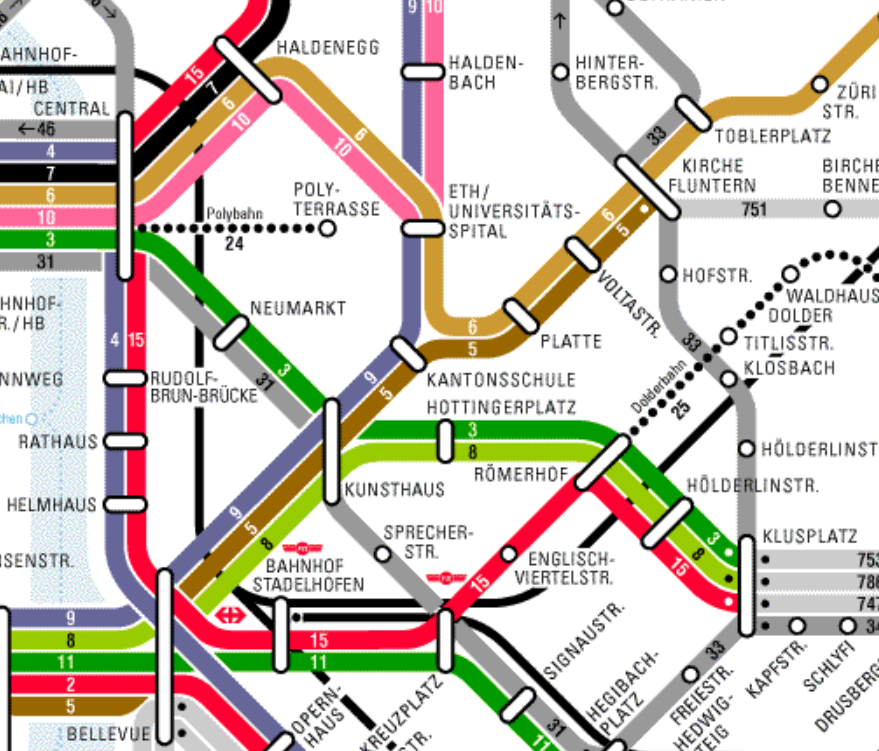
\includegraphics[width=\linewidth]{Pictures/Tram1.PNG}
    \caption{Ein Ausschnitt der Tram- und Buslinien in Zürich}
\end{figure}

Alice steht nach der Schule an der Haltestelle ''Kantonsschule'' in Zürich und möchte einen ganz bestimmten Kugelschreiber einkaufen gehen. Ihr Ziel ist es möglichst wenige Zwischenhaltestellen zu besuchen, bevor sie eine erreicht, in deren Nähe ein Laden mit dem genau diesem Kugelschreiber im Sortiment steht. Sie beginnt also zu überlegen: ''Die benachbarten Haltestellen sind\\ ''ETH/Universitätsspital'', ''Platte'' und ''Kunsthaus'', aber bei keiner dieser Stationen finde ich meinen Kugelschreiber. Nun kann ich von diesen drei Haltestellen wiederum für alle Benachbarten überlegen ob es dort den Kugelschreiber gibt, denn das sind genau jene Stationen die ich mit nur einem Zwischenstopp erreichen kann.'' Auf diese Art überlegt Alice weiter bis sie eine Haltestelle findet in deren Nähe der Kugelschreiber verkauft wird. \\

Das Problem der Suche nach dem Kugelschreiber können wir als Graph formalisieren, indem wir für jede Haltestelle einen Knoten zeichnen und jeweils die Benachbarten mit einer Kante verbinden. Alice beginnt also bei ihrem Startknoten ''Kantonsschule'' und durchläuft dann die restliche Knoten aufsteigend geordnet nach dem Abstand zu diesem Startknoten. Erinnere dich, dass wir den Abstand von zwei Knoten in einem Graphen definiert haben als die Anzahl Kanten des kürzesten Weges vom ersten Knoten zum zweiten. Das von Alice durchgeführte Vorgehen entspricht der Breitensuche, einem Algorithmus mit welchem wir uns in den folgenden 2 Lektionen befassen werden.\\

Nachdem wir im ersten Quartal die Grundlagen der Graphentheorie sowie das Implementieren von einfachen Algorithmen in Python gelernt haben, wollen wir jetzt diese beiden Themen vereinen indem wir mit der Breitensuche einen Algorithmus für Graphen betrachten. Am Ende dieser zwei Lektionen werdet ihr die Breitensuche für einen beliebigen Graphen selbst durchführen können und den Algorithmus auch in Python implementieren können. Ihr werdet erkennen wie vielfältig die Breitensuche angewendet werden kann und den Algorithmus und sein Programm an einige verschiedene Problemstellungen anpassen können.

Wir beginnen im nächsten Abschnitt damit, das genaue Vorgehen des Algorithmus zuerst in Worten und dann anhand einer Folge von Bildern durchzugehen. Zudem implementieren wir die Breteinsuche in Python. Anhand der zugehörigen Aufgaben lernst du bereits verschiedene mögliche Anwendungen kennen.  In Abschnitt 3 geht es darum die Breitensuche zu verwenden um kürzeste Pfade zwischen zwei bliebigen Knoten in einem Graphen zu finden.